\section{Time Series Analysis}
We decided to do task 4.1 as last part of the project which expected us to find groups of similar cities given their temperature trends.
\autoref{fig:timeseries_dataset} shows the initial dataset and the modified one, the latter, built with the pivot method from pandas, was the one we worked on during our analysis. The resulting dataframe now has the cities as indexes and the temperature records as values, so it made our task easier.

\begin{figure}[H]
    \centering
    \subfloat[Initial dataset]{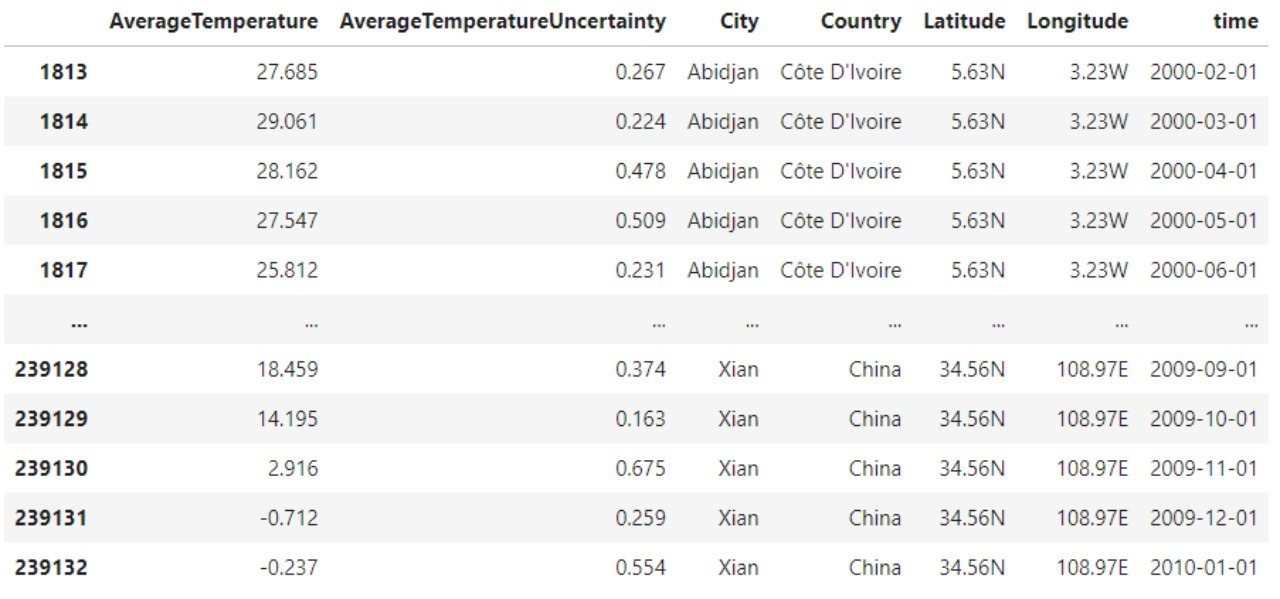
\includegraphics[width=0.38\linewidth]{images/time_series_analysis/timeseries_dataset.jpg}}
    \subfloat[The organized dataset]{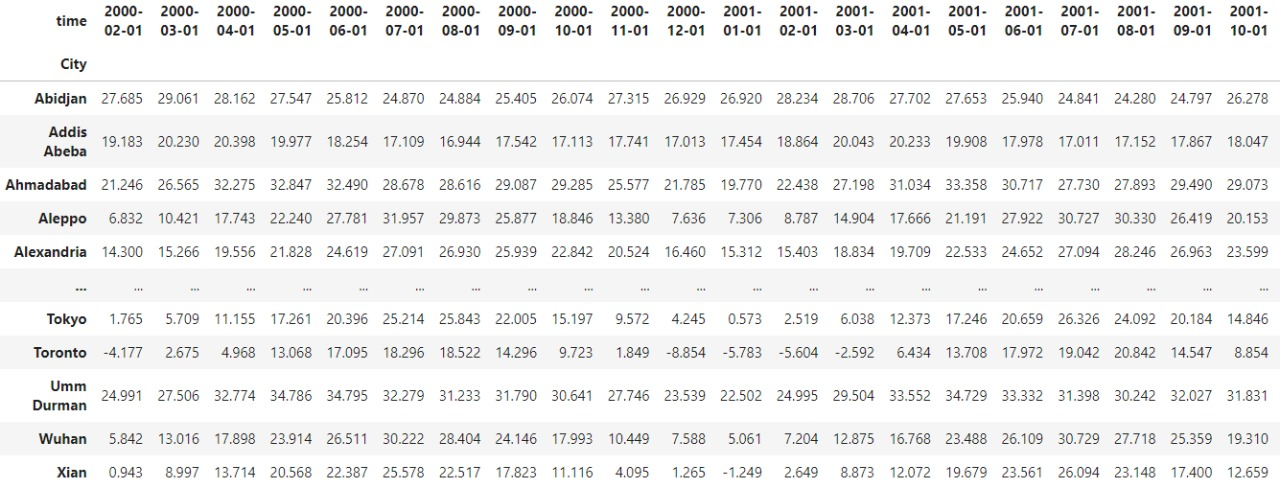
\includegraphics[width=0.48\linewidth]{images/time_series_analysis/timeseries_dataset_modified.jpg}}
    \caption{Time series dataset before and after using the pivot method from pandas.}
    \label{fig:timeseries_dataset}
\end{figure}

\subsection{Shape-based clustering}
We used the k-means clustering from the tslearn package to find those similar groups of cities and in order to choose the best values of k (the number of clusters) we based our choice, as seen during the clustering task, on the SSE, silhouette and Davies-Bouldin scores. Afterwards, we took the best k value and we used it to do the final clustering on the cities dataframe.
\begin{figure}[H]
    \centering
    \subfloat[Scores]{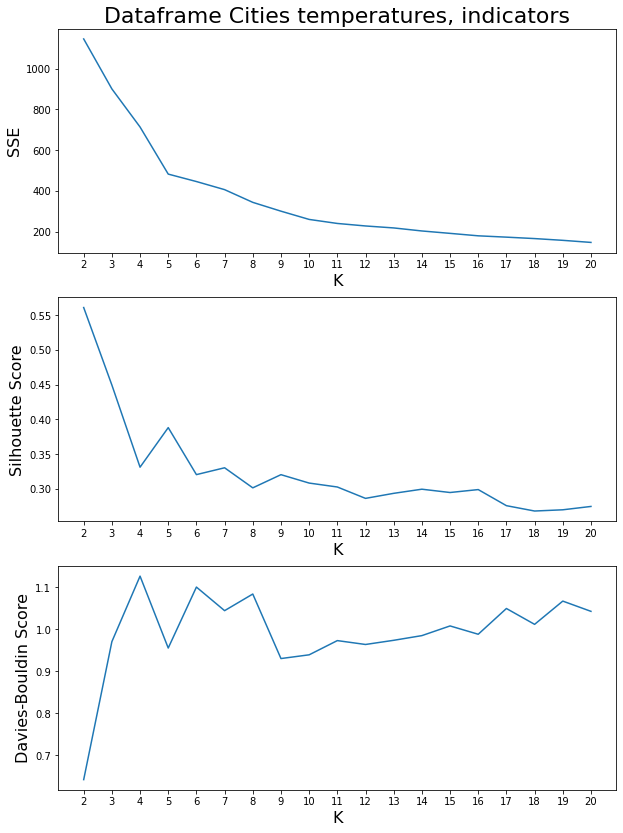
\includegraphics[width=0.28\linewidth]{images/time_series_analysis/timeseries_k.png}}
    \subfloat[The plot with k=5]{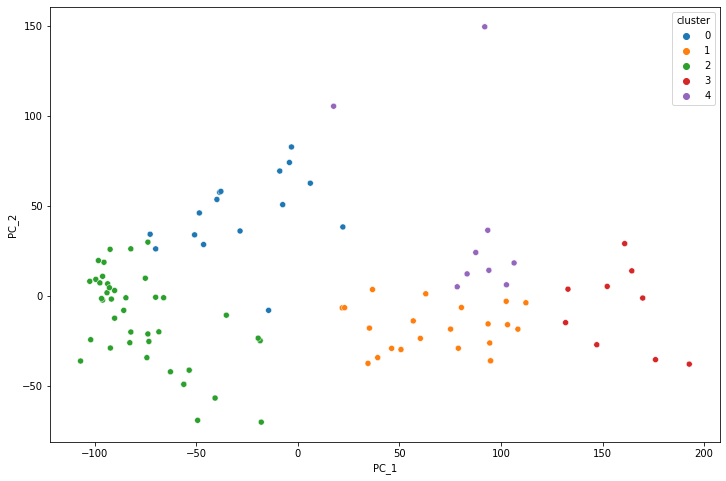
\includegraphics[width=0.4\linewidth]{images/time_series_analysis/timeseries_plot_clusters.png}}
    \caption{Scores for each value of k and clustering with the best k value.}
    \label{fig:timeseries_clusters}
\end{figure}
As \autoref{fig:timeseries_clusters} on the left shows, by using the elbow rule and by looking at the other two values we took 5 as the best value for k and the final clustering analysis is shown on \autoref{fig:timeseries_clusters} on the right end.
\vspace{3mm}

The cities are, therefore, separated in five different cluster in accordance to their temperature trends: \textit{warm winter and very hot summer}, \textit{cold winter and hot summer}, \textit{very hot winter and very hot summer}, \textit{warm winter and mild summer} and lastly \textit{very cold winter and mild summer}.
We then plotted those temperature trends on a graph in order to compare them between each other, the cities were, instead, plotted on a map according to the cluster they belong to.
\begin{figure}[H]
    \centering
    \subfloat[Cluster trends]{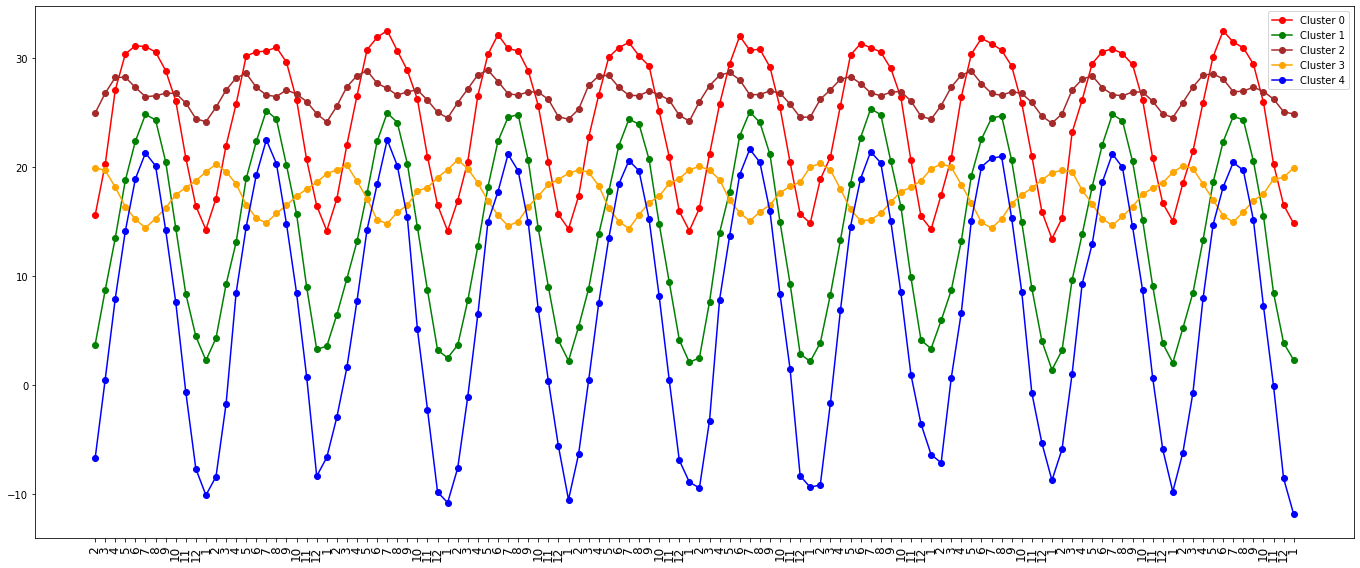
\includegraphics[width=0.41\linewidth]{images/time_series_analysis/timeseries_plot.png}}
    \subfloat[Cluster map]{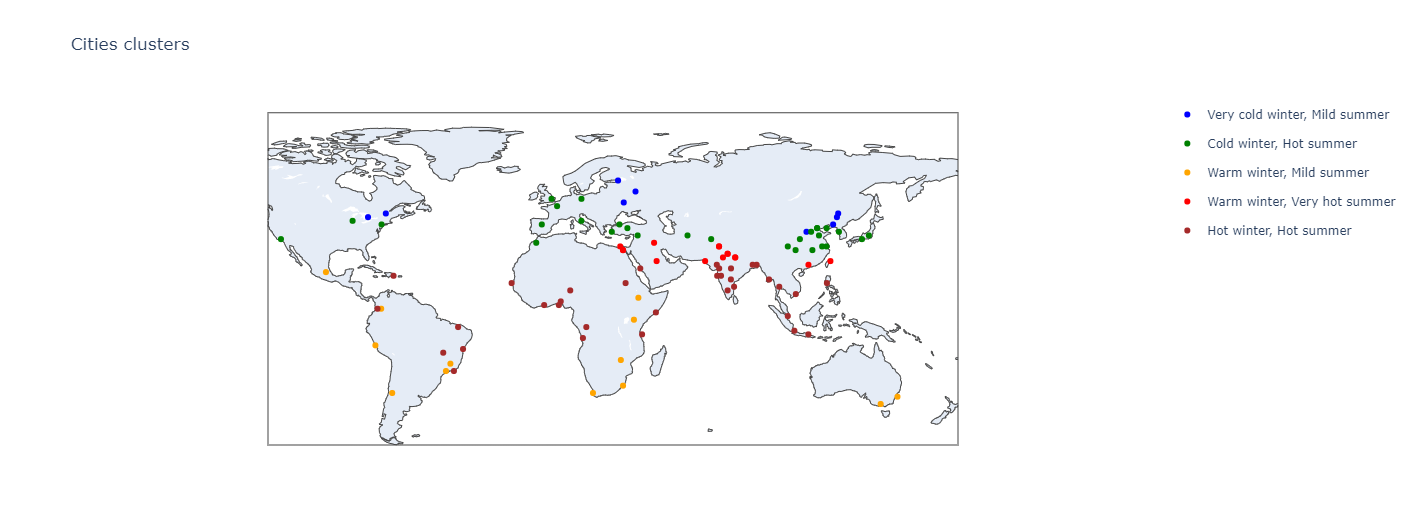
\includegraphics[width=0.59\linewidth]{images/time_series_analysis/timeseries_map.png}}
    \caption{Temperature trends for each cluster and the map with the cities plotted with respect to the cluster they belong to.}
    \label{fig:timeseries_plot_map}
\end{figure}
The map in \autoref{fig:timeseries_plot_map} shows that cities in similar clusters are somewhat at the same latitude (which is something that we expected).

\subsection{Feature-based clustering}
As final clustering analysis on the time series, we decided to try the feature-based approach by defining new features from the ones we had and by doing the same work that we did for the shape-based clustering. The features we built were based on the mean temperatures for each season (keep in mind that seasons are different in the two emispheres) and then we inserted the mean, max and min temperatures recorded for each city.
\begin{figure}[H]
    \centering
    \subfloat[Cluster trends]{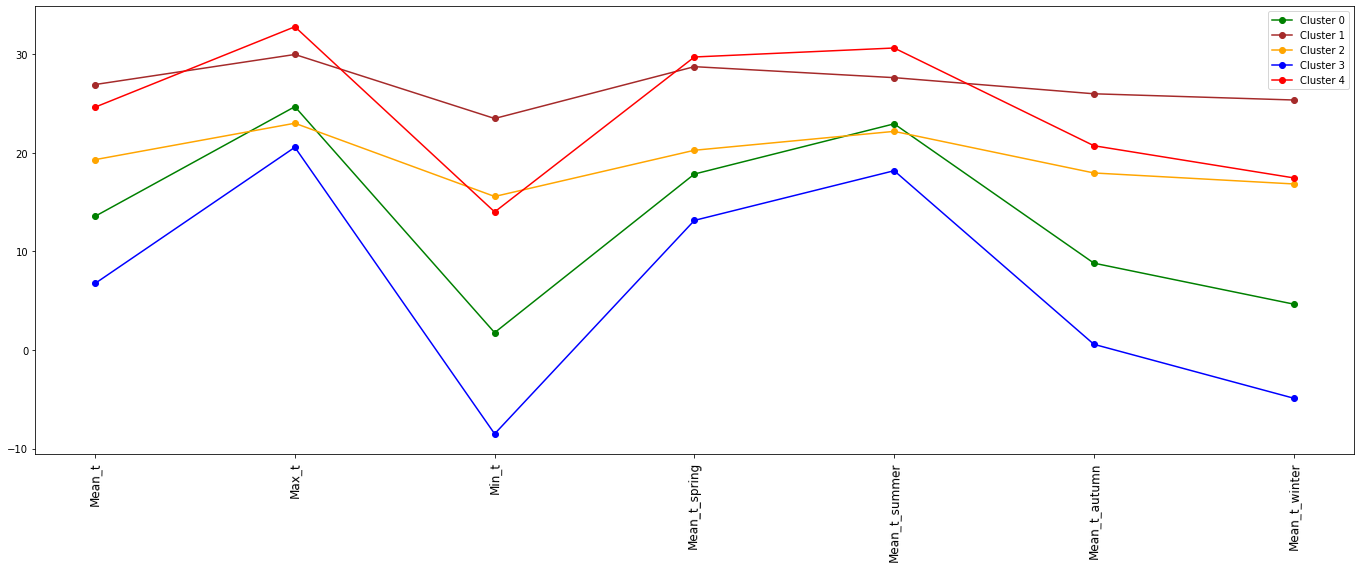
\includegraphics[width=0.41\linewidth]{images/time_series_analysis/timeseries_fbc_plot.png}}
    \subfloat[Cluster map]{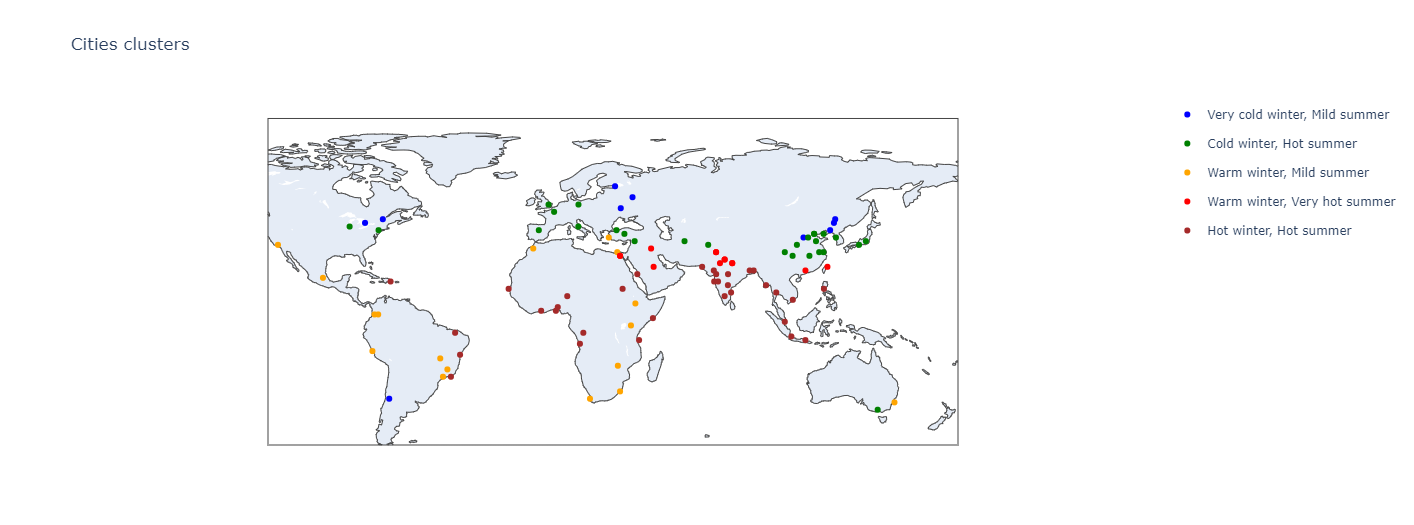
\includegraphics[width=0.59\linewidth]{images/time_series_analysis/timeseries_fbc_map.png}}
    \caption{Statistics for each cluster (our newly defined features) and the map with the cities plotted with respect to the cluster they belong to.}
    \label{fig:timeseries_fbc_plot_map}
\end{figure}
The results are pretty similar with respect to the shape-based approach since not many cities were classified in very different clusters.
